\section{Structural Operation Semantics}
The operational semantics is the rules that give our syntax meaning, and without them, it would be impossible to make a working language, as a given syntax wouldn't have a clearly defined functionality. For this reason, we will define the operational semantics in this section.

There are two common ways of describing the semantics of a language. Big-step semantics and small-step semantics. While they are mostly equivalent, there are some advantages and disadvantages to both of them. The big-step semantics evaluates the whole expression from the start to the end expression. Small-step semantics may only evaluate part of the expression one step at a time. The disadvantage of small-step semantics is that it can be daunting to both write and read.

We have decided to make our operational semantics a small-step semantics, as a small-step semantic ruleset is easier to extend in the case of a new feature compared to a big-step semantic ruleset. This means that it would be possible to add parallelity if we realize that we need it at a later date.

\subsection{Environment-Store Model}
To describe how the Ezuino compiler handle and store variables, we will use the environment store model. The different mechanisms in the environment store model will be described before starting on the semantics. First, we have the location, which marks the location of every variable value in the program. The location keeps track of a variable in the environment $env_v$.
To continue with the enviromental store model, we got the partial function named Store (Sto), which for an instance of the program binds its storage location to values, which are contained within. An example of this is that if we want to find the value of a specific variable, in this case, named x, we write $"sto \ env_v \ x"$.
Next, we have the run-time stack named envl. The runtime stack is a list of pairs ($env_v$, $env_p$).
In figure \ref{evnstoreexmp}, a illustration of the environment store model can be reviewed.
\begin{figure}[H]
\centering
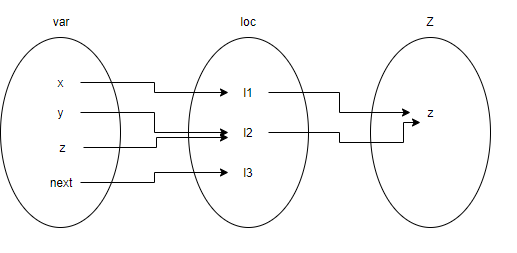
\includegraphics[scale=0.75]{figures/evnstore.png}
\caption{Environment Store Example}
\label{evnstoreexmp}
\end{figure}


\subsection{Arithmetic Expressions}
In the following table, it should be noted that most transitions will be on the form \( \langle envl, sto, a \rangle \Rightarrow_e \langle envl', sto', v \rangle \). This is supposed to be read as "By evaluating a in accord with the runtime stack and the store like an expression, a is evaluated to the value v, and the runtime stack and store is updated

\begin{longtable}[c] { r c }
  \centering
  
  [VAR] & \( envl, sto \vdash x \Rightarrow_e v \) \\
  & if \(env_v x = l \) \\
  & and \(sto \ l = v \) \\
  & where \(envl = (env_v, env_p) : envl' \) \\
  &  \\

  [DCL] & \( 
    \dfrac{ \langle D_V, envl[x \mapsto l][next \mapsto \text{new} \ l], sto \rangle \Rightarrow_{DV} \langle envl', sto \rangle}
    { \langle T x, envl, sto \rangle \Rightarrow_{DV} \langle envl', sto \rangle } \) \\
  & \\

  [PARENT-1] & 
    \( \dfrac { \langle e, envl, sto \rangle \Rightarrow_e \langle e', envl', sto' \rangle }
      { \langle (e), envl, sto \rangle  \Rightarrow_e \langle (e'), envl', sto' \rangle } \) \\
  & \\

  [PARENT-2] & 
    \( \langle (v), envl, sto \rangle \Rightarrow_e \langle v, envl, sto \rangle \) \\
  & \\

  [PLUS-1] & 
    \( \dfrac { \langle e_1, envl, sto \rangle \Rightarrow_e \langle e_1', envl', sto' \rangle )}
      {\langle e_1 + e_2, envl, sto \rangle \Rightarrow_e \langle e_1' + e_2, envl', sto' \rangle } \) \\
  & \\

  [PLUS-2] & 
    \( \dfrac { \langle e_2, envl, sto \rangle \Rightarrow_e \langle e_2', envl', sto' \rangle }
      {\langle v_1 + e_2, envl, sto \rangle  \Rightarrow_e \langle e_1 + e_2', envl', sto' \rangle } \) \\
  & \\

  [PLUS-3] & 
    \( \langle v_1 + v_2, envl, sto \rangle \Rightarrow \langle v, envl, sto \rangle \) \\
  & where \( v = v_1 + v_2\) \\
  & \\

  [MINUS-1] & 
    \( \dfrac { \langle e_1, envl, sto \rangle \Rightarrow_e \langle e_1', envl', sto' \rangle }
      {\langle e_1 - e_2, envl, sto \rangle \Rightarrow_e \langle e_1' - e_2, envl', sto' \rangle } \) \\
  & \\

  [MINUS-2] & 
    \( \dfrac { \langle e_2, envl, sto \rangle \Rightarrow_e \langle e_2', envl', sto' \rangle }
      {\langle v_1 - e_2, envl, sto \rangle \Rightarrow_e \langle v_1 - e_2', envl', sto' \rangle } \) \\
  & \\

  [MINUS-3] & 
    \( \langle v_1 - v_2, envl, sto \rangle \Rightarrow \langle v, envl, sto \rangle \) \\
  & where \( v = v_1 - v_2\) \\
  & \\

  [MULT-1] & 
    \( \dfrac { \langle e_1, envl, sto \rangle \Rightarrow_e \langle e_1', envl', sto' \rangle }
      {\langle e_1 * e_2, envl, sto \rangle \Rightarrow_e \langle e_1' * e_2, envl', sto' \rangle } \) \\
  & \\

  [MULT-2] & 
    \( \dfrac { \langle e_2, envl, sto \rangle \Rightarrow_e \langle e_2', envl', sto' \rangle }
      {\langle v_1 * e_2, envl, sto \rangle \Rightarrow_e \langle v_1 * e_2', envl', sto' \rangle } \) \\
  & \\

  [MULT-3] & 
    \( \langle v_1 * v_2, envl, sto \rangle \Rightarrow \langle v, envl, sto \rangle \) \\
  & where \( v = v_1 * v_2\) \\
  & \\

  [DIV-1] & 
    \( \dfrac { \langle e_1, envl, sto \rangle \Rightarrow_e \langle e_1', envl', sto' \rangle }
      {\langle e_1 / e_2, envl, sto \rangle \Rightarrow_e \langle e_1' / e_2, envl', sto' \rangle } \) \\
  & \\

  [DIV-2] & 
    \( \dfrac { \langle e_2, envl, sto \rangle \Rightarrow_e \langle e_2', envl', sto' \rangle }
      {\langle v_1 / e_2, envl, sto \rangle \Rightarrow_e \langle v_1 / e_2', envl', sto' \rangle } \) \\
  & \\

  [DIV-3] & 
    \( \langle v_1 / v_2, envl, sto \rangle \Rightarrow \langle v, envl, sto \rangle \) \\
  & where \( v = \dfrac{ v_1 }{ v_2 } \) \\
  & \\

  [NEGATION-1] & 
    \( \dfrac { \langle e_1, envl, sto \rangle \Rightarrow_e \langle e_1', envl', sto' \rangle }
      {\langle -e_1, envl, sto \rangle \Rightarrow_e \langle -e_1', envl', sto' \rangle } \) \\
  & \\

  [NEGATION-2] & 
    \( \langle -v_1, envl, sto \rangle \Rightarrow \langle v, envl, sto \rangle \) \\
  & where \( v = -v_1 \)\\
  & \\

  [NUM] & 
    \( n \Rightarrow v \) \\
  & \( \text{if } \mathcal{N} [[n]] = v \) \\

  \caption{Small-step semantics for arithmetic expressions}
\end{longtable}

\subsection{Boolean Expressions}
\begin{longtable}[c] { r c }
  \centering
  [NOT-1] & \( 
    \dfrac { \langle e, envl, sto \rangle \Rightarrow_e \langle e', envl', sto' \rangle }
      { \langle !e, envl, sto \rangle \Rightarrow_e \langle !e', envl', sto' \rangle } \)
  \\
  & \\

  [NOT-TRUE] & \( 
    \langle !v, envl, sto \rangle \Rightarrow_e \langle tt, envl, sto \rangle \)
  \\
  & if \( v = ff\) \\
  & \\

  [NOT-FALSE] & \( 
    \langle !v, envl, sto \rangle \Rightarrow_e \langle ff, envl, sto \rangle \)
  \\
  & if \( v = tt \) \\
  & \\

  [AND-1] & \( 
    \dfrac { \langle e_1, envl, sto \rangle \Rightarrow_e \langle e_1', envl', sto' \rangle }
      { \langle e_1 \ AND \ e_2, envl, sto \rangle \Rightarrow_e \langle e_1' \ AND \ e_2, envl', sto' \rangle } \)
  \\
  & \\

  [AND-2] & \( 
    \dfrac { \langle e_2, envl, sto \rangle \Rightarrow_e \langle e_2', envl', sto' \rangle }
      { \langle v_1 \ AND \ e_2, envl, sto \rangle \Rightarrow_e \langle v_1 \ AND \ e_2', envl', sto' \rangle } \)
  \\
  & \\

  [AND-3] & \( 
    \langle v_1 \ AND \ v_2, envl, sto \rangle \Rightarrow_e \langle tt, envl, sto \rangle \)
  \\
  & if \( v_1 \land v_2 \) \\
  & \\

  [AND-4] & \( 
    \langle v_1 \ AND \ v_2, envl, sto \rangle \Rightarrow_e \langle ff, envl, sto \rangle \)
  \\
  & if \( \neg(v_1 \land v_2) \) \\
  & \\

  [OR-1] & \( 
    \dfrac { \langle e_1, envl, sto \rangle \Rightarrow_e \langle e_1', envl', sto' \rangle }
      { \langle e_1 \ OR \ e_2, envl, sto \rangle \Rightarrow_e \langle e_1' \ OR \ e_2, envl', sto' \rangle } \)
  \\
  & \\

  [OR-2] & \( 
    \dfrac { \langle e_2, envl, sto \rangle \Rightarrow_e \langle e_2', envl', sto' \rangle }
      { \langle v_1 \ OR \ e_2, envl, sto \rangle \Rightarrow_e \langle v_1 \ OR \ e_2', envl', sto' \rangle } \)
  \\
  & \\

  [OR-3] & \( 
    \langle v_1 \ OR \ v_2, envl, sto \rangle \Rightarrow_e \langle tt, envl, sto \rangle \)
  \\
  & if \( v_1 \lor v_2 \) \\
  & \\

  [OR-4] & \( 
    \langle v_1 \ OR \ v_2, envl, sto \rangle \Rightarrow_e \langle ff, envl, sto \rangle \)
  \\
  & if \( \neg(v_1 \lor  v_2) \) \\
  & \\

  [EQUAL-1] & \( 
    \dfrac { \langle e_1, envl, sto \rangle \Rightarrow_e \langle e_1', envl', sto' \rangle }
      { \langle e_1 = e_2, envl, sto \rangle \Rightarrow_e \langle e_1' = e_2, envl', sto' \rangle } \)
  \\
  & \\

  [EQUAL-2] & \( 
    \dfrac { \langle e_2, envl, sto \rangle \Rightarrow_e \langle e_2', envl', sto' \rangle }
      { \langle v_1 = e_2, envl, sto \rangle \Rightarrow_e \langle v_1 = e_2', envl', sto' \rangle } \)
  \\
  & \\

  [EQUAL-3] & \( 
    \langle v_1 = v_2, envl, sto \rangle \Rightarrow_e \langle tt, envl, sto \rangle \)
  \\
  & if \( v_1 = v_2 \) \\
  & \\

  [EQUAL-4] & \( 
    \langle v_1 = v_2, envl, sto \rangle \Rightarrow_e \langle ff, envl, sto \rangle \)
  \\
  & if \( \neg(v_1 = v_2) \) \\
  & \\

  [NOT-EQUAL-1] & \( 
    \dfrac { \langle e_1, envl, sto \rangle \Rightarrow_e \langle e_1', envl', sto' \rangle }
      { \langle e_1 != e_2, envl, sto \rangle \Rightarrow_e \langle e_1' != e_2, envl', sto' \rangle } \)
  \\
  & \\

  [NOT-EQUAL-2] & \( 
    \dfrac { \langle e_2, envl, sto \rangle \Rightarrow_e \langle e_2', envl', sto' \rangle }
      { \langle v_1 != e_2, envl, sto \rangle \Rightarrow_e \langle v_1 != e_2', envl', sto' \rangle } \)
  \\
  & \\

  [NOT-EQUAL-3] & \( 
    \langle v_1 != v_2, envl, sto \rangle \Rightarrow_e \langle tt, envl, sto \rangle \)
  \\
  & if \( \neg(v_1 = v_2) \) \\
  & \\

  [NOT-EQUAL-4] & \( 
    \langle v_1 != v_2, envl, sto \rangle \Rightarrow_e \langle ff, envl, sto \rangle \)
  \\
  & if \( v_1 = v_2 \) \\
  & \\

  [GREATER-THAN-1] & \( 
    \dfrac { \langle e_1, envl, sto \rangle \Rightarrow_e \langle e_1', envl', sto' \rangle }
      { \langle e_1 > e_2, envl, sto \rangle \Rightarrow_e \langle e_1' > e_2, envl', sto' \rangle } \)
  \\
  & \\

  [GREATER-THAN-2] & \( 
    \dfrac { \langle e_2, envl, sto \rangle \Rightarrow_e \langle e_2', envl', sto' \rangle }
      { \langle v_1 > e_2, envl, sto \rangle \Rightarrow_e \langle v_1 > e_2', envl', sto' \rangle } \)
  \\
  & \\

  [GREATER-THAN-3] & \( 
    \langle v_1 > v_2, envl, sto \rangle \Rightarrow_e \langle tt, envl, sto \rangle \)
  \\
  & if \( v_1 > v_2 \) \\
  & \\

  [GREATER-THAN-4] & \( 
    \langle v_1 > v_2, envl, sto \rangle \Rightarrow_e \langle ff, envl, sto \rangle \)
  \\
  & if \( \neg(v_1 > v_2) \) \\
  & \\

  [GREATER-THAN-OR-EQUAL-1] & \( 
    \dfrac { \langle e_1, envl, sto \rangle \Rightarrow_e \langle e_1', envl', sto' \rangle }
      { \langle e_1 > = e_2, envl, sto \rangle \Rightarrow_e \langle e_1' > = e_2, envl', sto' \rangle } \)
  \\
  & \\

  [GREATER-THAN-OR-EQUAL-2] & \( 
    \dfrac { \langle e_2, envl, sto \rangle \Rightarrow_e \langle e_2', envl', sto' \rangle }
      { \langle v_1 > = e_2, envl, sto \rangle \Rightarrow_e \langle v_1 > = e_2', envl', sto' \rangle } \)
  \\
  & \\

  [GREATER-THAN-OR-EQUAL-3] & \( 
    \langle v_1 > = v_2, envl, sto \rangle \Rightarrow_e \langle tt, envl, sto \rangle \)
  \\
  & if \( v_1 \geq v_2 \) \\
  & \\

  [GREATER-THAN-OR-EQUAL-4] & \( 
    \langle v_1 > = v_2, envl, sto \rangle \Rightarrow_e \langle ff, envl, sto \rangle \)
  \\
  & if \( \neg(v_1 \geq v_2) \) \\
  & \\

  [LESS-THAN-1] & \( 
    \dfrac { \langle e_1, envl, sto \rangle \Rightarrow_e \langle e_1', envl', sto' \rangle }
      { \langle e_1 < e_2, envl, sto \rangle \Rightarrow_e \langle e_1' < e_2, envl', sto' \rangle } \)
  \\
  & \\

  [LESS-THAN-2] & \( 
    \dfrac { \langle e_2, envl, sto \rangle \Rightarrow_e \langle e_2', envl', sto' \rangle }
      { \langle v_1 < e_2, envl, sto \rangle \Rightarrow_e \langle v_1 < e_2', envl', sto' \rangle } \)
  \\
  & \\

  [LESS-THAN-3] & \( 
    \langle v_1 < v_2, envl, sto \rangle \Rightarrow_e \langle tt, envl, sto \rangle \)
  \\
  & if \( v_1 < v_2 \) \\
  & \\

  [LESS-THAN-4] & \( 
    \langle v_1 < v_2, envl, sto \rangle \Rightarrow_e \langle ff, envl, sto \rangle \)
  \\
  & if \( \neg(v_1 < v_2) \) \\
  & \\

  [LESS-THAN-OR-EQUAL-1] & \( 
    \dfrac { \langle e_1, envl, sto \rangle \Rightarrow_e \langle e_1', envl', sto' \rangle }
      { \langle e_1 < = e_2, envl, sto \rangle \Rightarrow_e \langle e_1' < = e_2, envl', sto' \rangle } \)
  \\
  & \\

  [LESS-THAN-OR-EQUAL-2] & \( 
    \dfrac { \langle e_2, envl, sto \rangle \Rightarrow_e \langle e_2', envl', sto' \rangle }
      { \langle v_1 < = e_2, envl, sto \rangle \Rightarrow_e \langle v_1 < = e_2', envl', sto' \rangle } \)
  \\
  & \\

  [LESS-THAN-OR-EQUAL-3] & \( 
    \langle v_1 < = v_2, envl, sto \rangle \Rightarrow_e \langle tt, envl, sto \rangle \)
  \\
  & if \( v_1 \leq v_2 \) \\
  & \\

  [LESS-THAN-OR-EQUAL-4] & \( 
    \langle v_1 < = v_2, envl, sto \rangle \Rightarrow_e \langle ff, envl, sto \rangle \)
  \\
  & if \( \neg(v_1 \leq v_2) \) \\
  & \\
  \caption{Small-step semantics boolean expressions}
\end{longtable}
\subsection{Boolean Expressions}
\begin{table}[H]
    \centering
    \begin{longtable}[c] { r c }
    \begin{tabular}{@{}c@{}} 
    [ASS1] &
    \\
    \\
    \end{tabular}
  \begin{tabular}{@{}c@{}}   \( <x := a, sto, env_l> \Rightarrow (sto[l -> v], envl) \)  \\ \( env_v,sto \vdash n \Rightarrow v \)
  \\ \( env_v,sto \vdash n \Rightarrow v \)
  \end{tabular}
        
 \end{longtable}
    \caption{Small-step semantics for boolean assignment expressions}\label{tab:my_label}
\end{table}
        
\begin{table}[H]
    \centering
    \begin{longtable}[c] { r c }
        
        [IF-ELSE-TRUE] & \( \dfrac{\langle \texttt{if} \ b \ \texttt{then} \ S_1 \ \texttt{else} \ S_2,\ s \rangle \Rightarrow \langle S_1,\ s\rangle}{if\ s\vdash b \rightarrow_b tt} \) \\[4ex]
        
        [IF-ELSE-FALSE] & \( \dfrac{\langle \texttt{if} \ b \ \texttt{then} \ S_1 \ \texttt{else} \ S_2,\ s \rangle \Rightarrow \langle S_2,\ s \rangle}{if\ s\vdash b \rightarrow_b ff} \) \\[4ex]
        
        [IF-TRUE] & \( \dfrac{\langle \texttt{if} \ b \ \texttt{then} \ S_1,\ s \rangle \Rightarrow \langle S_1,\ s \rangle}{if \ s\vdash b \rightarrow_b tt} \) \\\\
        
        [IF-FALSE] & \( \dfrac{\langle \texttt{if} \ b \ \texttt \ S_1,\ s \rangle \Rightarrow s}{if\ s\vdash b \rightarrow_b ff} \) \\[4ex]
        
 \end{longtable}
    \caption{Small-step semantics for boolean if statement}\label{tab:my_label}
\end{table}
        
\begin{table}[H]
    \centering
    \begin{longtable}[c] { r c }
        
        [WHILE] & \( \langle \texttt{while(} \ b\texttt{) \{} S \texttt{\}},\ s \rangle \Rightarrow \langle \texttt{if} \ b \ \texttt{then} (S\texttt{;while (} b \texttt{) \{} S\texttt{\}}) \texttt{else skip,}\ s\rangle) \) \\[4ex]
        
 \end{longtable}
    \caption{Small-step semantics for boolean while statements}\label{tab:my_label}
\end{table}
        
\begin{table}[H]
    \centering
    \begin{longtable}[c] { r c }
    
        [END] & END\\
    \end{longtable}
    \caption{Small-step semantics for end}\label{tab:my_label}
\end{table}